\chapter{7 TeV and 8 TeV Differential Cross Section Measurement}

During 2011 and 2012, the LHC produced millions of top quark pair events with gluon-gluon fusion (\~70\%) or
quark\-anti\-quark annihilation (\~30\%) being the primary production mechanisms. Top quarks decay almost
100\% of the time to a W-boson and a b flavour jet. The W-boson then decays either hadronically (into two
jets) or leptonically (lepton + neutrino). Top pair events are characterised by the decay of the W-bosons:
\begin{itemize}
  \item Leptonic - both W-bosons decay to a lepton and a neutrino. The event would consist of 6 jets.
  \item Hadronic - both W-bosons decay to two jets. The event would consist of 2 jets, 2 leptons and 2
  neutrinos (which would show up as \met in the event).
  \item Semi-Leptonic - one W-boson decays to a lepton and a neutrino, the other decays to two jets. The
  event would consist of 4 jets, 1 lepton and 1 neutrino.
\end{itemize}

This analysis investigates the semi-leptonic channel and was carried out on 2011 and 2012 data recorded from
the CMS detector. A measurement of the normalised differential \ttbar cross section with
respect to the following global variables is carried out:
\begin {itemize}
  \item {\met, the missing transverse energy in an event}
  \item {\HT, the sum of the jet transverse momenta in an event}
  \item {\st, the sum of the observed transverse momenta in an event}
  \item {\mt, the transverse mass of the leptonically decaying W boson}
  \item {\wpt, the transverse momentum of the leptonically decaying W boson}
\end{itemize}

Previous analyses using 7~TeV data investigating \met and using 8~TeV data investigatin all the global
variables listed above can be found in \cite{CMS-PAS-TOP-12-019} and \cite{CMS-PAS-TOP-12-042} respectively.

This investigation is motivated primarily by the importance of understanding \ttbar events since they are a
significant background in many new physics analyses. It is also helpful in understanding QCD and event
generators. Rare Standard Model processes such as $\ttbar + W\rightarrow l\nu$ or $\ttbar + Z\rightarrow
\nu\bar{\nu}$ would appear in \met distribution tail, and $\ttbar + X$ where $X$ is massive would appear in
the \HT and \st distributions. There are also possible new physics scenarios such as stop pair production,
$\tilde{t}\bar{\tilde{t}} \rightarrow t\tilde{\chi_0} \bar{t}\bar{\tilde{\chi_0}}$ could show hints of dark
matter, rare Standard Model processes etc.

A simultaneous fit is done with three templates in bins of each variable.
The binning choice is made based on two variables: purity (equation) and stability (equation). The purity of a
bin is sensitive to events moving into/out of a bin and the stability is sensitive to events moving inout/out
of a bin. The bins for each global variable are selected such that each bin has purity and stability values of
0.5 or greater, meaning that at least half of the events created in a bin remain in that bin.
	
Electrons can be faked by jets, so the electron scale factors could be different in ttbar events than in
events from which the scale factors were derived because our events contain a lot more activity than events
from which the scale factors were derived.
For muons it is not so bad because muons leave a much cleaner signal inside CMS and there is no risk of jets
faking muons.
	
We use the lepton trigger, identification and isolation scale factors provided by the Muon POG for both 7 TeV
and 8 TeV. However, for electrons, although we have 8 TeV scale factors provided by the EGamma POG, we have
had to derive scale factors ourselves for 7 TeV because not provided (and the trigger we use is not included
in the 7 TeV Summer 11 Legacy datasets).
The hadronic leg of the electronHad trigger needs to be measured in relation to the 4 jets. ASK ABOUT THIS
	 
Remember:
- V\_Jets template combined over all global variable bins.
- QCD template also inclusive over all global variable bins
	
	
	
Within the framework of this analysis, prompt leptons are considered as those which come
from W or Z boson or from tau-lepton decays. These leptons are usually well isolated, whereas
misidentified leptons originate either from semi-leptonic heavy flavor decays within jets or are
simply misreconstructed genuine jets. In both cases these leptons are generally not isolated.



Tau energy: The met energy systematics are electron energy up/down, muon energy up/down and tau energy
up/down. These systematics (and JES) are applied to both monte carlo and data. We found that the tau energy is
susprisingly high, considerably higher than the electron and muon energy systematics. We may select taus in
our signal region unintentionally although we don't select on taus. The signature of ttbar events with taus
can mimic the signature of electron + jets or muon + jets ttbar events. The image shows how taus decay. The W
from a top could decay to a tau, which would then decay either to a tau neutrino and a virtual W which then
decays to two jets which would be very close together (and therefore reconstructed as a single jet). Or, the
virtual W could decay to a lepton (electron or muon) and an associated neutrino). These signatures could fake
our signal, and therefore end up in our ttbar signal. In our unfolding, we remove fakes. However, we use the
shape of the fakes in the central to subtract from the signal distribution in the tau energy up/down
variations. The effect is not so pronounced in the electron up/down and muon up/down variations because there
are not many electrons or muons in the fakes. Luke found that \~14\% of the TTJet events we select on are NOT
from the decay we are looking for. This was by dividing the number of events in the fake ST distribution in
the unfolding histogram file by the number of events in the measured distribution (i.e. signal) in the same
file. Th electron channel was actually ~13.5\% and the muon channel was actually ~13.9\%. The shape
comparison between the fakes and the signal shows that there are more fakes in the higher MET bins, which is
why the error in those bins is larger. These are likely to come from semi-leptonic tau events (where the tau
decays to a lepton and a neutrino); tau tau, e tau or mu tau where the tau decays hadronically; or ee, emu or mumu events where one of the leptons is lost (probably low fraction as well). So most of our fakes will include at least one tau. Since semi-leptonic tau would need to
decay leptonically, these taus are not identified and, I assume, not included in the MET uncertainty.

Looking at the shape difference between the central and tau up/down MET distributions, there is a significant
different (though not by much). Since this affects data, the difference goes through the fit, and the
unfolding, and is what we see in the final result. The difference in normalisation in the most affected bin is
\~6\%, suggesting that we have more than 6\% tau contamination overall (not sure if that is a correct
assumption). The normalisation across the bins does not change, of course, i.e. the sum of events in the bins
of, in this case MET, remain the same in the central measurement and in the tau energy up/down variations.
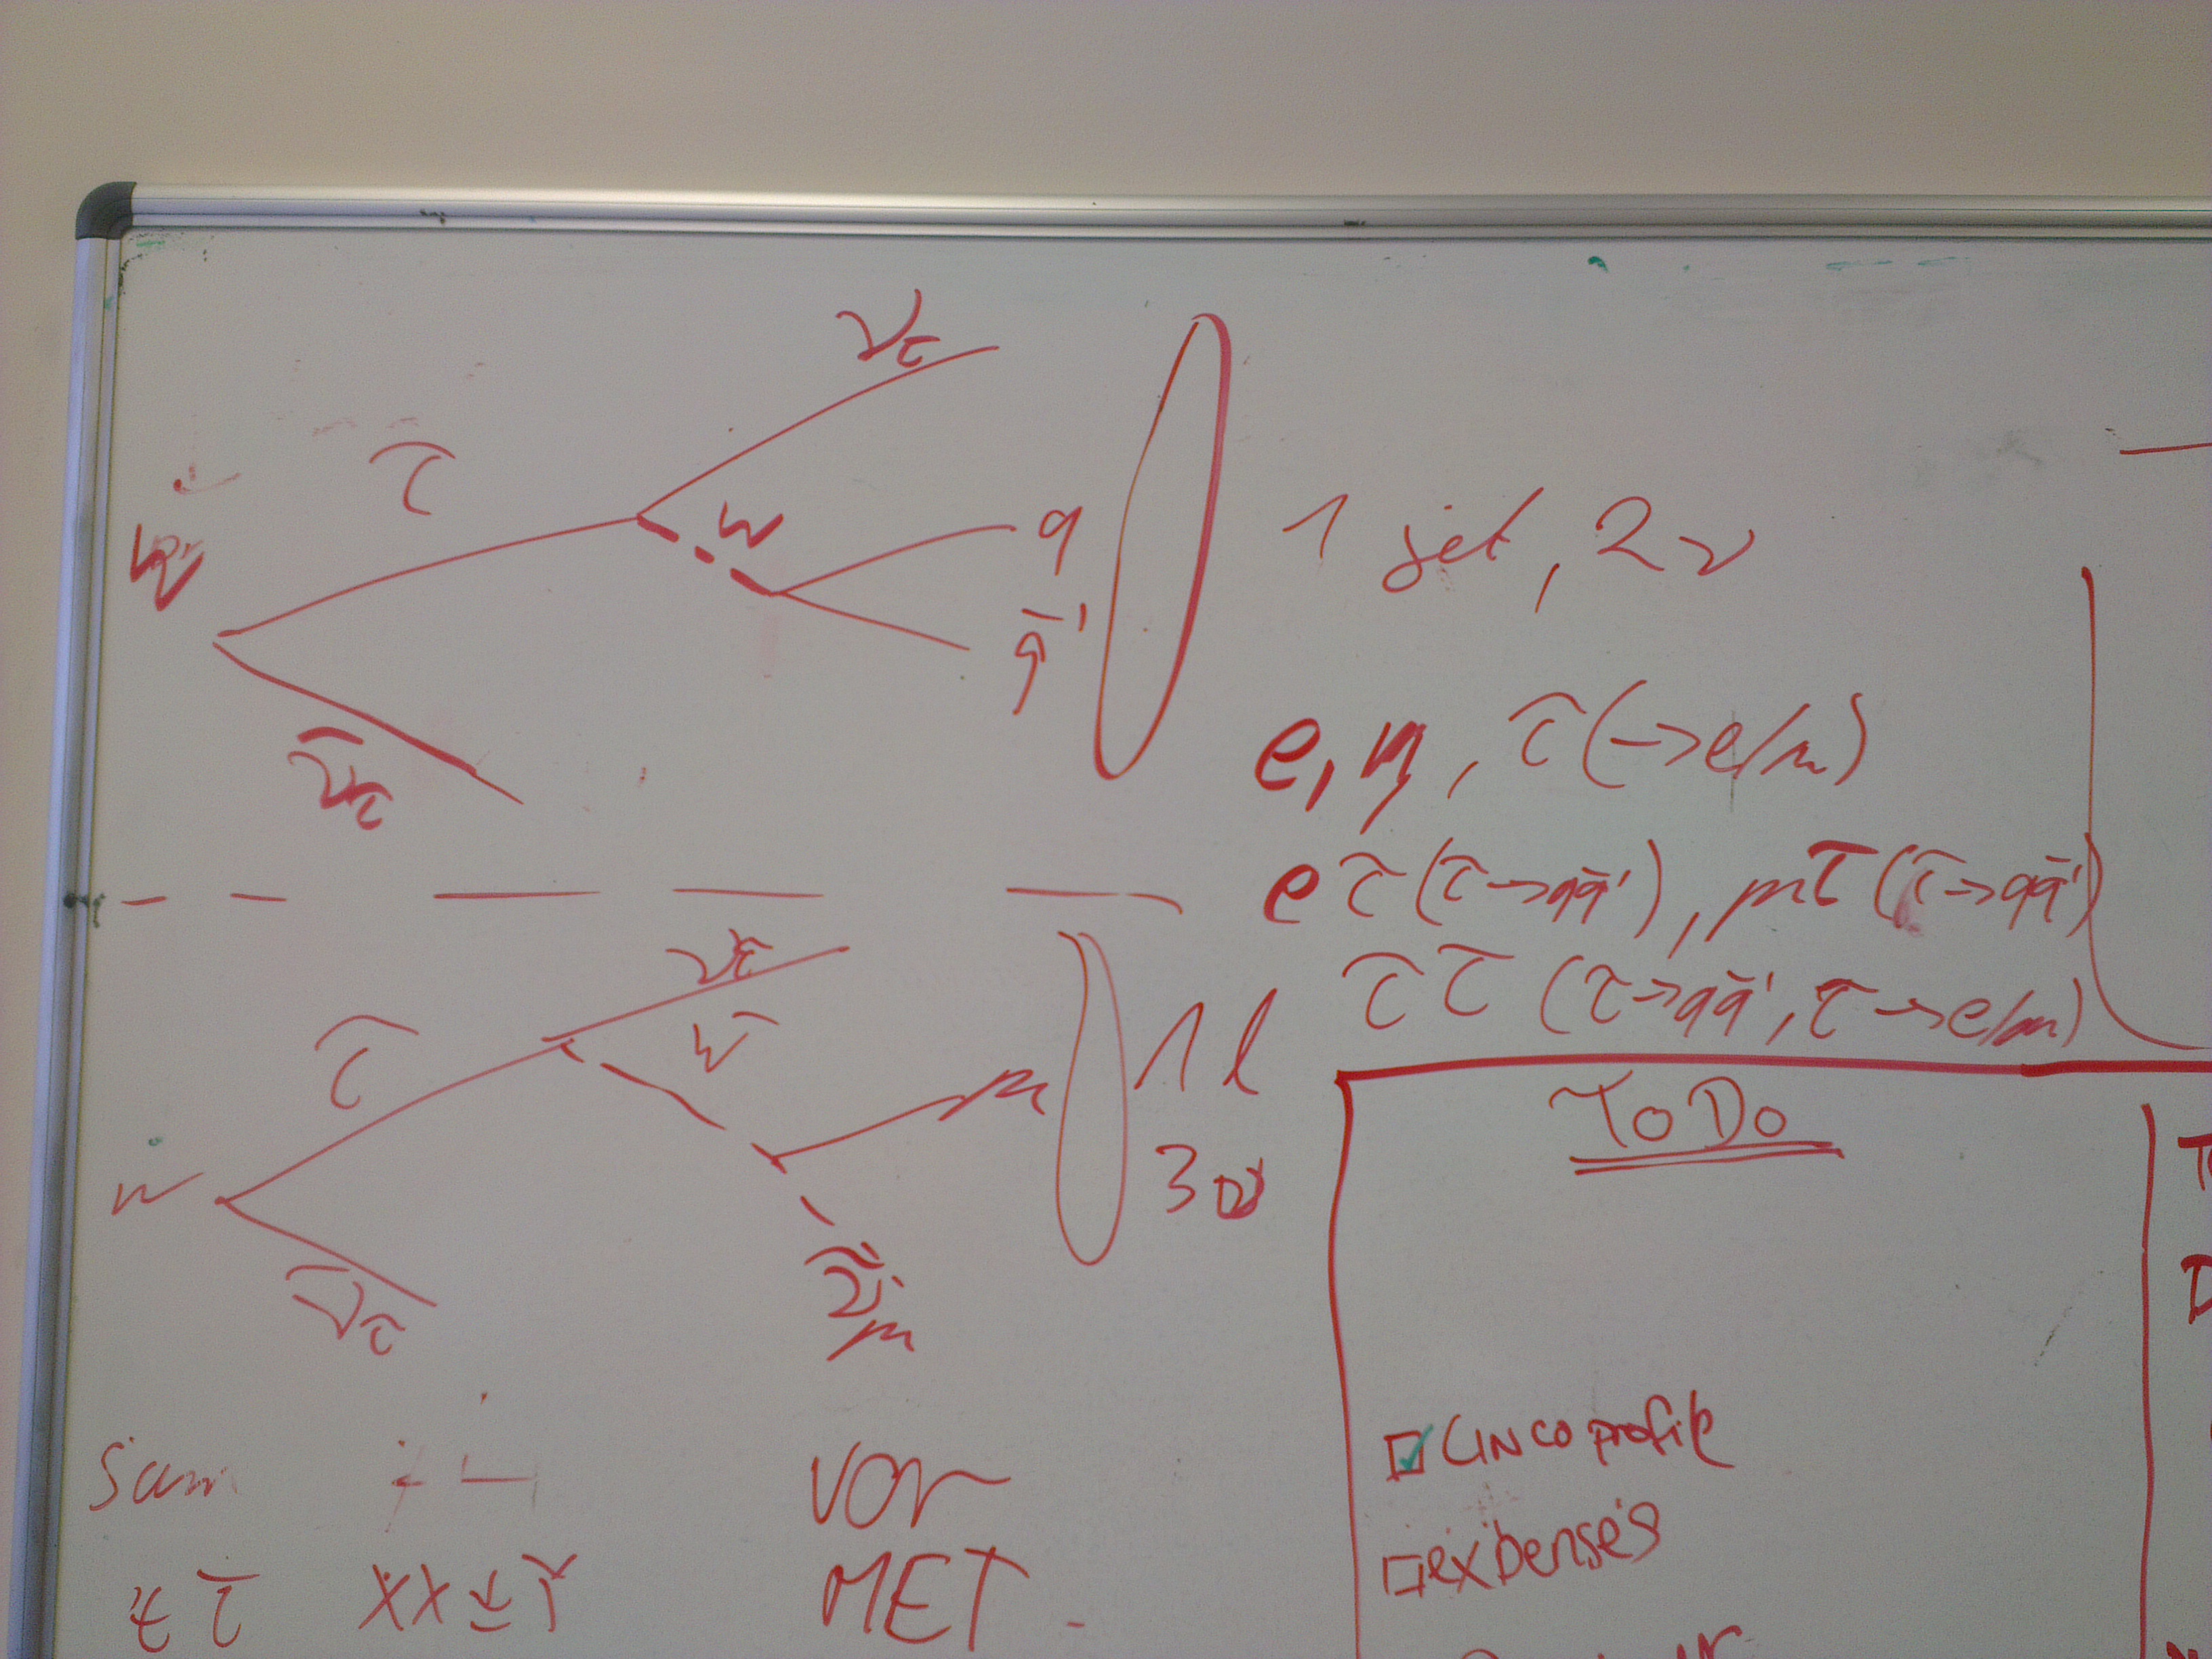
\includegraphics[width=\textwidth]{Chapters/04_Analysis/Images/IMG_20150219_160840.jpg}
